\documentclass[a4paper,man,11pt,floatsintext]{apa6}
%\documentclass[a4paper,man,11pt,floatsintext]{apa7}

% ------------------------------------------------------------------------------
% Document settings
% ------------------------------------------------------------------------------
% jou = journal style, i.e. 2 columns
% man = manuscript style for submissions

% floatsintext = figures and tables remain at their intended position in the text. Delete it if you want them to occur at the end of the manuscript.

% ------------------------------------------------------------------------------
% Find the full documentation for apa6/7 package here:
% ------------------------------------------------------------------------------

% https://ctan.kako-dev.de/macros/latex/contrib/apa6/apa6.pdf
% https://ctan.mc1.root.project-creative.net/macros/latex/contrib/apa7/apa7.pdf

% ------------------------------------------------------------------------------
% Additional packages
% ------------------------------------------------------------------------------
\usepackage[american]{babel}
\usepackage{csquotes}
\usepackage[style=apa6,sortcites=true,sorting=nyt,backend=biber]{biblatex}
\usepackage{nameref}
% ------------------------------------------------------------------------------
% Import .bib-file
% ------------------------------------------------------------------------------
\addbibresource{../refs/library.bib}
% ------------------------------------------------------------------------------
% Title page
% ------------------------------------------------------------------------------
\title{I am a very exciting title}
\shorttitle{Insert running head here}

% APA 7 version
%\authorsnames[{1,2},{1,2}]{Auth1, Auth2}
%\authorsaffiliations{
%{Institute of Whatsoever, University of Nowhere},
%{Institute of Something Else, Another University}
%}
%\authornote{
%Corresponding author:\\
%Auth1 \\
%Mail: *** \\
%Phone: ***
%}
%\leftheader{Auth1 & Auth2 202*} for jou mode only

% APA 6 version
\author{Auth1$^{1,2}$ and Auth2$^{1,2}$}
\affiliation{
$^{1}$Institute of Whatsoever, University of Nowhere \\
$^{2}$Institute of Something Else, Another University
}
\authornote{
Corresponding author:\\
Auth1 \\
Mail: *** \\
Phone: ***
}
%\leftheader{Auth1 \& Auth2 202*} %for jou mode only

% ------------------------------------------------------------------------------
% Abstract
% ------------------------------------------------------------------------------
\abstract{I am a convincing abstract...}
\keywords{key1, key2, key3, ...}
% ------------------------------------------------------------------------------
% Begin document
% ------------------------------------------------------------------------------
\begin{document}
\maketitle
% Import some external .tex documents
\section{Introduction}

Let's cite \textcite{Michel2021} to showcase how citation commands are used \parencite[also works in parentheses][]{Michel2021}. Figure \ref{fig:fig1} shows an APA figure example.


\begin{figure}[!ht]
    \centering
    \caption{}
    \label{fig:fig1}
    \caption*{\textit{APA Requires The Title Above The Figure}}
    \vspace*{8mm}
    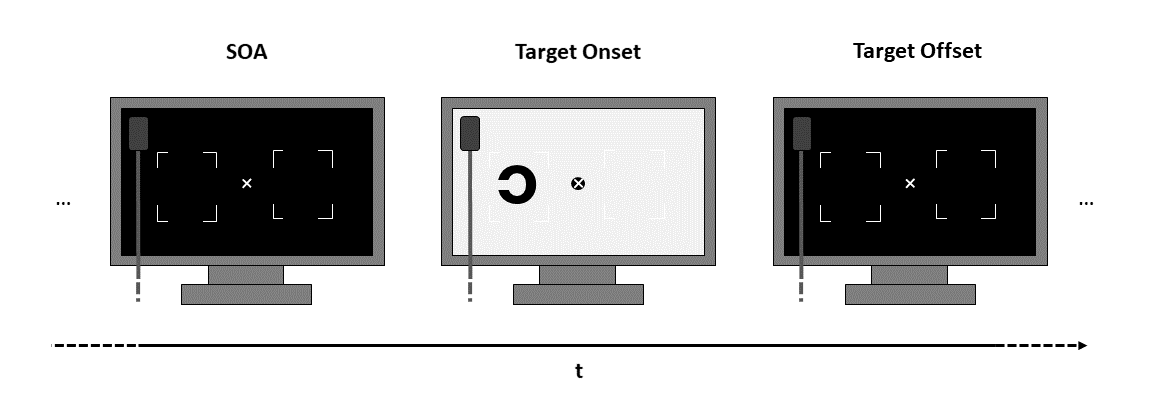
\includegraphics[width=1\textwidth]{../figures/Fig1}
    \caption*{\textit{Note.} Here you can add all your notes regarding the figure.}
\end{figure}

\section{Study 1}

\subsection{Methods}

\subsubsection{Participants}

Describe your sample here. Below you can find a random equation

\begin{equation}
f = \sqrt{\frac{\eta_{p}^{2}}{1-\eta_{p}^{2}}}
\end{equation}

which I only added to intimidate the reader of the template.

\subsubsection{Material}

Here I will briefly describe the material of the study.

\paragraph{Apparatus}
VPixx here, Eyelink there...The typical paragraph to skip when you read a paper.


\paragraph{Stimuli}
Just a description of our typical lines and circles, i.e. the puristic beauty of psychophysics.


 \subsection{Results}

Table \ref{tab:models} shows some intimidating formulas in an APA-style table. I deeply hope that there is another (and more straightforward) way to set up a table, because tables in LaTeX are a nightmare...

\begin{table}[htbp]
  \centering
  \vspace*{2em}
  \begin{threeparttable}
    \caption{Just some formulas}
    \label{tab:models}
    \begin{tabular}{@{}lc@{}}
      \toprule
        \multicolumn{1}{c}{\textbf{model}}  & \multicolumn{1}{c}{\textbf{formula}} \\
      \midrule
        intercept model & \multicolumn{1}{c}{$f(t) = b_{0}$} \\
        linear model &   \multicolumn{1}{c}{$f(t) = b_{0} + b_{1}t$} \\
      \midrule
    \end{tabular}
    \begin{tablenotes}[para,flushleft]
      {\small\textit{Note.} $b_{0,1}$ = beta weights,  $t$ = time.}
    \end{tablenotes}
  \end{threeparttable}
\end{table}

Just some random text below the table to create the illusion of a real manuscript. Nothing important to say here.


\section*{Funding}
\label{funding}
This study is supported by ***.

\section*{Conflict of interest}
\label{coi}
The authors declare no competing financial interests.

\section*{Ethical approval}
\label{ethics}
The study was conducted in accordance with the ethical standards laid down in the World Medical Association Declaration of Helsinki \parencite{WorldMedicalAssociation2013}.

\section*{Author Contributions}
\label{contrib}
Auth1 did whatsoever. Auth2 did something else.

\printbibliography

\end{document}
